\documentclass[tikz,border=2pt]{standalone}
\usepackage{amsmath}
\usepackage{pgfplots}
\pgfplotsset{compat=1.18}

\begin{document}
% 0 <= a_n <= b_n term by term: if the larger terms b_n have a convergent sum, so do the a_n
% (their partial sums are increasing and bounded by the sum of the b_n).
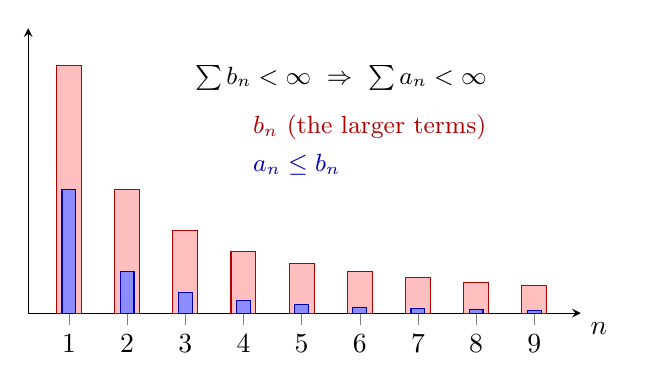
\begin{tikzpicture}
	\begin{axis}[
		axis lines=middle,
		xmin=0.3, xmax=9.8,
		ymin=0, ymax=1.15,
		xtick={1,...,9}, ytick=\empty,
		xlabel={$n$}, ylabel={},
		xlabel style={below right},
		ybar, bar width=9pt, bar shift=0pt,
		clip=false,
		width=8.6cm, height=5.2cm
		]
		\addplot[fill=red!25, draw=red!70!black, samples at={1,...,9}] {1/x};
		\addplot[fill=blue!45, draw=blue!70!black, bar width=5pt, samples at={1,...,9}] {1/(x*(x+1))};
		\node[red!70!black, anchor=west, font=\small] at (axis cs:4,0.75) {$b_n$ (the larger terms)};
		\node[blue!70!black, anchor=west, font=\small] at (axis cs:4,0.6) {$a_n\le b_n$};
		\node[anchor=west, font=\small] at (axis cs:3,0.95) {$\sum b_n<\infty\ \Rightarrow\ \sum a_n<\infty$};
	\end{axis}
\end{tikzpicture}
\end{document}
